% Generated by Sphinx.
\def\sphinxdocclass{report}
\documentclass[letterpaper,10pt,english]{sphinxmanual}
\usepackage[utf8]{inputenc}
\DeclareUnicodeCharacter{00A0}{\nobreakspace}
\usepackage{cmap}
\usepackage[T1]{fontenc}
\usepackage{babel}
\usepackage{times}
\usepackage[Bjarne]{fncychap}
\usepackage{longtable}
\usepackage{sphinx}
\usepackage{multirow}



\title{Sensum Documentation}
\date{November 24, 2014}
\release{1.2}
\author{Daniel Aurelio Galeazzo}
\newcommand{\sphinxlogo}{}
\renewcommand{\releasename}{Release}
\makeindex

\makeatletter
\def\PYG@reset{\let\PYG@it=\relax \let\PYG@bf=\relax%
    \let\PYG@ul=\relax \let\PYG@tc=\relax%
    \let\PYG@bc=\relax \let\PYG@ff=\relax}
\def\PYG@tok#1{\csname PYG@tok@#1\endcsname}
\def\PYG@toks#1+{\ifx\relax#1\empty\else%
    \PYG@tok{#1}\expandafter\PYG@toks\fi}
\def\PYG@do#1{\PYG@bc{\PYG@tc{\PYG@ul{%
    \PYG@it{\PYG@bf{\PYG@ff{#1}}}}}}}
\def\PYG#1#2{\PYG@reset\PYG@toks#1+\relax+\PYG@do{#2}}

\expandafter\def\csname PYG@tok@gd\endcsname{\def\PYG@tc##1{\textcolor[rgb]{0.63,0.00,0.00}{##1}}}
\expandafter\def\csname PYG@tok@gu\endcsname{\let\PYG@bf=\textbf\def\PYG@tc##1{\textcolor[rgb]{0.50,0.00,0.50}{##1}}}
\expandafter\def\csname PYG@tok@gt\endcsname{\def\PYG@tc##1{\textcolor[rgb]{0.00,0.27,0.87}{##1}}}
\expandafter\def\csname PYG@tok@gs\endcsname{\let\PYG@bf=\textbf}
\expandafter\def\csname PYG@tok@gr\endcsname{\def\PYG@tc##1{\textcolor[rgb]{1.00,0.00,0.00}{##1}}}
\expandafter\def\csname PYG@tok@cm\endcsname{\let\PYG@it=\textit\def\PYG@tc##1{\textcolor[rgb]{0.25,0.50,0.56}{##1}}}
\expandafter\def\csname PYG@tok@vg\endcsname{\def\PYG@tc##1{\textcolor[rgb]{0.73,0.38,0.84}{##1}}}
\expandafter\def\csname PYG@tok@m\endcsname{\def\PYG@tc##1{\textcolor[rgb]{0.13,0.50,0.31}{##1}}}
\expandafter\def\csname PYG@tok@mh\endcsname{\def\PYG@tc##1{\textcolor[rgb]{0.13,0.50,0.31}{##1}}}
\expandafter\def\csname PYG@tok@cs\endcsname{\def\PYG@tc##1{\textcolor[rgb]{0.25,0.50,0.56}{##1}}\def\PYG@bc##1{\setlength{\fboxsep}{0pt}\colorbox[rgb]{1.00,0.94,0.94}{\strut ##1}}}
\expandafter\def\csname PYG@tok@ge\endcsname{\let\PYG@it=\textit}
\expandafter\def\csname PYG@tok@vc\endcsname{\def\PYG@tc##1{\textcolor[rgb]{0.73,0.38,0.84}{##1}}}
\expandafter\def\csname PYG@tok@il\endcsname{\def\PYG@tc##1{\textcolor[rgb]{0.13,0.50,0.31}{##1}}}
\expandafter\def\csname PYG@tok@go\endcsname{\def\PYG@tc##1{\textcolor[rgb]{0.20,0.20,0.20}{##1}}}
\expandafter\def\csname PYG@tok@cp\endcsname{\def\PYG@tc##1{\textcolor[rgb]{0.00,0.44,0.13}{##1}}}
\expandafter\def\csname PYG@tok@gi\endcsname{\def\PYG@tc##1{\textcolor[rgb]{0.00,0.63,0.00}{##1}}}
\expandafter\def\csname PYG@tok@gh\endcsname{\let\PYG@bf=\textbf\def\PYG@tc##1{\textcolor[rgb]{0.00,0.00,0.50}{##1}}}
\expandafter\def\csname PYG@tok@ni\endcsname{\let\PYG@bf=\textbf\def\PYG@tc##1{\textcolor[rgb]{0.84,0.33,0.22}{##1}}}
\expandafter\def\csname PYG@tok@nl\endcsname{\let\PYG@bf=\textbf\def\PYG@tc##1{\textcolor[rgb]{0.00,0.13,0.44}{##1}}}
\expandafter\def\csname PYG@tok@nn\endcsname{\let\PYG@bf=\textbf\def\PYG@tc##1{\textcolor[rgb]{0.05,0.52,0.71}{##1}}}
\expandafter\def\csname PYG@tok@no\endcsname{\def\PYG@tc##1{\textcolor[rgb]{0.38,0.68,0.84}{##1}}}
\expandafter\def\csname PYG@tok@na\endcsname{\def\PYG@tc##1{\textcolor[rgb]{0.25,0.44,0.63}{##1}}}
\expandafter\def\csname PYG@tok@nb\endcsname{\def\PYG@tc##1{\textcolor[rgb]{0.00,0.44,0.13}{##1}}}
\expandafter\def\csname PYG@tok@nc\endcsname{\let\PYG@bf=\textbf\def\PYG@tc##1{\textcolor[rgb]{0.05,0.52,0.71}{##1}}}
\expandafter\def\csname PYG@tok@nd\endcsname{\let\PYG@bf=\textbf\def\PYG@tc##1{\textcolor[rgb]{0.33,0.33,0.33}{##1}}}
\expandafter\def\csname PYG@tok@ne\endcsname{\def\PYG@tc##1{\textcolor[rgb]{0.00,0.44,0.13}{##1}}}
\expandafter\def\csname PYG@tok@nf\endcsname{\def\PYG@tc##1{\textcolor[rgb]{0.02,0.16,0.49}{##1}}}
\expandafter\def\csname PYG@tok@si\endcsname{\let\PYG@it=\textit\def\PYG@tc##1{\textcolor[rgb]{0.44,0.63,0.82}{##1}}}
\expandafter\def\csname PYG@tok@s2\endcsname{\def\PYG@tc##1{\textcolor[rgb]{0.25,0.44,0.63}{##1}}}
\expandafter\def\csname PYG@tok@vi\endcsname{\def\PYG@tc##1{\textcolor[rgb]{0.73,0.38,0.84}{##1}}}
\expandafter\def\csname PYG@tok@nt\endcsname{\let\PYG@bf=\textbf\def\PYG@tc##1{\textcolor[rgb]{0.02,0.16,0.45}{##1}}}
\expandafter\def\csname PYG@tok@nv\endcsname{\def\PYG@tc##1{\textcolor[rgb]{0.73,0.38,0.84}{##1}}}
\expandafter\def\csname PYG@tok@s1\endcsname{\def\PYG@tc##1{\textcolor[rgb]{0.25,0.44,0.63}{##1}}}
\expandafter\def\csname PYG@tok@gp\endcsname{\let\PYG@bf=\textbf\def\PYG@tc##1{\textcolor[rgb]{0.78,0.36,0.04}{##1}}}
\expandafter\def\csname PYG@tok@sh\endcsname{\def\PYG@tc##1{\textcolor[rgb]{0.25,0.44,0.63}{##1}}}
\expandafter\def\csname PYG@tok@ow\endcsname{\let\PYG@bf=\textbf\def\PYG@tc##1{\textcolor[rgb]{0.00,0.44,0.13}{##1}}}
\expandafter\def\csname PYG@tok@sx\endcsname{\def\PYG@tc##1{\textcolor[rgb]{0.78,0.36,0.04}{##1}}}
\expandafter\def\csname PYG@tok@bp\endcsname{\def\PYG@tc##1{\textcolor[rgb]{0.00,0.44,0.13}{##1}}}
\expandafter\def\csname PYG@tok@c1\endcsname{\let\PYG@it=\textit\def\PYG@tc##1{\textcolor[rgb]{0.25,0.50,0.56}{##1}}}
\expandafter\def\csname PYG@tok@kc\endcsname{\let\PYG@bf=\textbf\def\PYG@tc##1{\textcolor[rgb]{0.00,0.44,0.13}{##1}}}
\expandafter\def\csname PYG@tok@c\endcsname{\let\PYG@it=\textit\def\PYG@tc##1{\textcolor[rgb]{0.25,0.50,0.56}{##1}}}
\expandafter\def\csname PYG@tok@mf\endcsname{\def\PYG@tc##1{\textcolor[rgb]{0.13,0.50,0.31}{##1}}}
\expandafter\def\csname PYG@tok@err\endcsname{\def\PYG@bc##1{\setlength{\fboxsep}{0pt}\fcolorbox[rgb]{1.00,0.00,0.00}{1,1,1}{\strut ##1}}}
\expandafter\def\csname PYG@tok@kd\endcsname{\let\PYG@bf=\textbf\def\PYG@tc##1{\textcolor[rgb]{0.00,0.44,0.13}{##1}}}
\expandafter\def\csname PYG@tok@ss\endcsname{\def\PYG@tc##1{\textcolor[rgb]{0.32,0.47,0.09}{##1}}}
\expandafter\def\csname PYG@tok@sr\endcsname{\def\PYG@tc##1{\textcolor[rgb]{0.14,0.33,0.53}{##1}}}
\expandafter\def\csname PYG@tok@mo\endcsname{\def\PYG@tc##1{\textcolor[rgb]{0.13,0.50,0.31}{##1}}}
\expandafter\def\csname PYG@tok@mi\endcsname{\def\PYG@tc##1{\textcolor[rgb]{0.13,0.50,0.31}{##1}}}
\expandafter\def\csname PYG@tok@kn\endcsname{\let\PYG@bf=\textbf\def\PYG@tc##1{\textcolor[rgb]{0.00,0.44,0.13}{##1}}}
\expandafter\def\csname PYG@tok@o\endcsname{\def\PYG@tc##1{\textcolor[rgb]{0.40,0.40,0.40}{##1}}}
\expandafter\def\csname PYG@tok@kr\endcsname{\let\PYG@bf=\textbf\def\PYG@tc##1{\textcolor[rgb]{0.00,0.44,0.13}{##1}}}
\expandafter\def\csname PYG@tok@s\endcsname{\def\PYG@tc##1{\textcolor[rgb]{0.25,0.44,0.63}{##1}}}
\expandafter\def\csname PYG@tok@kp\endcsname{\def\PYG@tc##1{\textcolor[rgb]{0.00,0.44,0.13}{##1}}}
\expandafter\def\csname PYG@tok@w\endcsname{\def\PYG@tc##1{\textcolor[rgb]{0.73,0.73,0.73}{##1}}}
\expandafter\def\csname PYG@tok@kt\endcsname{\def\PYG@tc##1{\textcolor[rgb]{0.56,0.13,0.00}{##1}}}
\expandafter\def\csname PYG@tok@sc\endcsname{\def\PYG@tc##1{\textcolor[rgb]{0.25,0.44,0.63}{##1}}}
\expandafter\def\csname PYG@tok@sb\endcsname{\def\PYG@tc##1{\textcolor[rgb]{0.25,0.44,0.63}{##1}}}
\expandafter\def\csname PYG@tok@k\endcsname{\let\PYG@bf=\textbf\def\PYG@tc##1{\textcolor[rgb]{0.00,0.44,0.13}{##1}}}
\expandafter\def\csname PYG@tok@se\endcsname{\let\PYG@bf=\textbf\def\PYG@tc##1{\textcolor[rgb]{0.25,0.44,0.63}{##1}}}
\expandafter\def\csname PYG@tok@sd\endcsname{\let\PYG@it=\textit\def\PYG@tc##1{\textcolor[rgb]{0.25,0.44,0.63}{##1}}}

\def\PYGZbs{\char`\\}
\def\PYGZus{\char`\_}
\def\PYGZob{\char`\{}
\def\PYGZcb{\char`\}}
\def\PYGZca{\char`\^}
\def\PYGZam{\char`\&}
\def\PYGZlt{\char`\<}
\def\PYGZgt{\char`\>}
\def\PYGZsh{\char`\#}
\def\PYGZpc{\char`\%}
\def\PYGZdl{\char`\$}
\def\PYGZhy{\char`\-}
\def\PYGZsq{\char`\'}
\def\PYGZdq{\char`\"}
\def\PYGZti{\char`\~}
% for compatibility with earlier versions
\def\PYGZat{@}
\def\PYGZlb{[}
\def\PYGZrb{]}
\makeatother

\renewcommand\PYGZsq{\textquotesingle}

\begin{document}

\maketitle
\tableofcontents
\phantomsection\label{index::doc}


Welcome to the Sensum Earth Observation Tools documentation.


\chapter{Structure}
\label{index:sensum-earth-observation}\label{index:structure}\begin{description}
\item[{The Sensum Earth Observations Tools are made of two main sections, library and scripts:}] \leavevmode\begin{enumerate}
\item {} 
The Sensum Library is composed by 11 python modules  contain all functions, classes and structures and other developing stuffs.

\item {} 
The Sensum Script is the core of the project including all the algorithms developed to extract the vulnerability indicators; the ``script/'' folder contains all the python scripts with the main algoritms.

\end{enumerate}

\end{description}


\chapter{Installation Guide}
\label{index:installation-guide}

\section{Installation Guide}
\label{install::doc}\label{install:installation-guide}

\subsection{Library Installation}
\label{install:library-installation}

\subsubsection{Microsoft Windows}
\label{install:microsoft-windows}
You can choose between 32bit or 64bit installation depending on your machine.
\begin{description}
\item[{\textbf{All required downloads}}] \leavevmode\begin{description}
\item[{from \href{https://www.python.org/downloads/windows/}{https://www.python.org/downloads/windows/}}] \leavevmode\begin{enumerate}
\item {} 
python 2.7.x Windows x86 MSI installer (32bit) or Windows x86-64 MSI installer (64bit)

\end{enumerate}

\item[{from \href{http://www.lfd.uci.edu/~gohlke/pythonlibs/}{http://www.lfd.uci.edu/\textasciitilde{}gohlke/pythonlibs/} you need to choose between py2.7.exe (32bit) or amd64-py2.7.exe extensions.}] \leavevmode\begin{enumerate}
\setcounter{enumi}{1}
\item {} 
Scipy-stack-14.x

\item {} 
scikit-image-0.x

\item {} 
scikit-learn-0.x

\item {} 
ephem-3.x

\end{enumerate}

\item[{from \href{http://trac.osgeo.org/osgeo4w/}{http://trac.osgeo.org/osgeo4w/}:}] \leavevmode\begin{enumerate}
\setcounter{enumi}{5}
\item {} 
OSGeo4W network installer (32bit or 64bit)

\end{enumerate}

\end{description}

\item[{\textbf{Installation}}] \leavevmode\begin{enumerate}
\item {} 
Install all the executables in sequence.

\item {} \begin{description}
\item[{In OSGeo4w network installer select advanced installation}] \leavevmode\begin{quote}

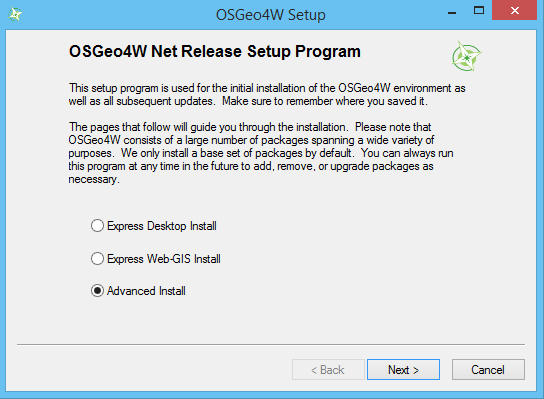
\includegraphics{advanced.png}
\end{quote}
\begin{description}
\item[{and add the following packages:}] \leavevmode\begin{itemize}
\item {} 
otb-bin

\item {} 
otb-python

\item {} 
qgis: QGIS Desktop

\end{itemize}

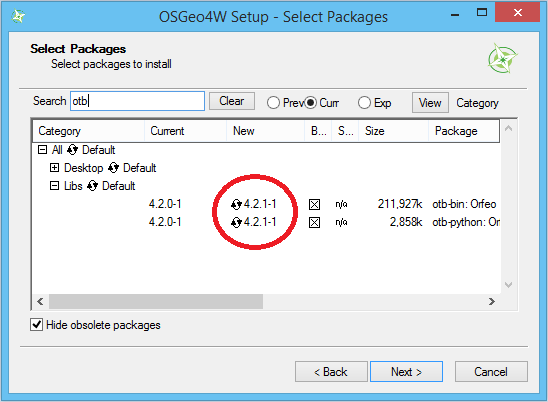
\includegraphics{select_packages.png}

\end{description}

\end{description}

\item {} \begin{description}
\item[{Go to Control Panel, System, Windows Advanced System Settings and set the following Environment Variable:}] \leavevmode\begin{itemize}
\item {} 
Variable name: PYTHONPATH

\item {} 
Variable value: C:/Python27/Lib/site-packages;C:/OSGeo4W64/apps/Python27/Lib/site-packages (for 64bit) or C:/Python27/Lib/site-packages;C:/OSGeo4W/apps/Python27/Lib/site-packages (for 32bit)

\end{itemize}

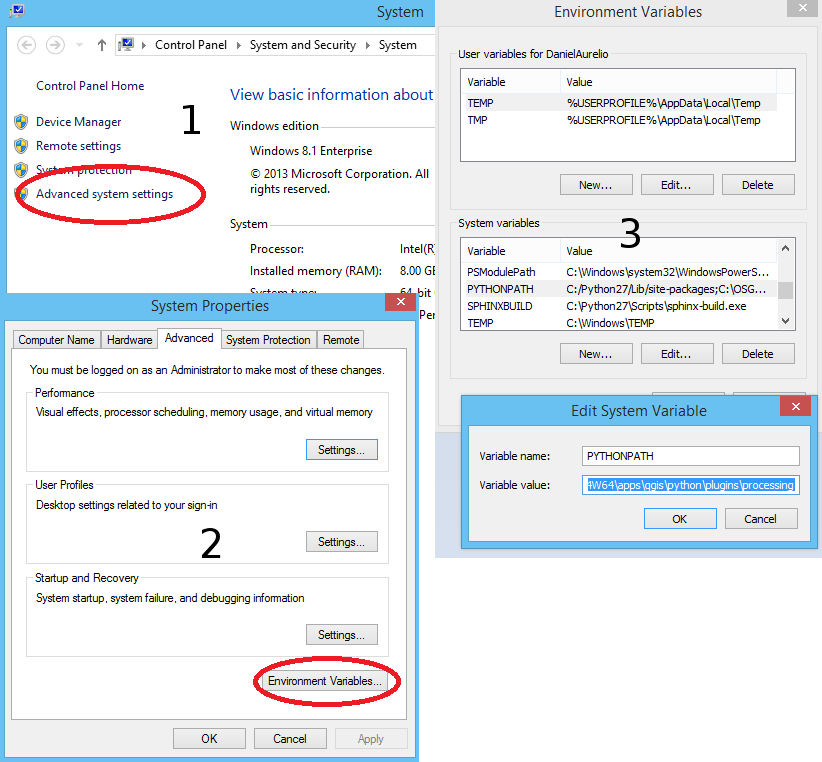
\includegraphics{set_variable.png}

\end{description}

\end{enumerate}

\end{description}


\subsubsection{Ubuntu/Debian}
\label{install:ubuntu-debian}\begin{description}
\item[{\textbf{Gdal, OpenCV, Sklearn, Skimage, QGIS, PyEphem Installation}}] \leavevmode
Procedure to install all the required software in a few steps; open your terminal and type the following code:

\begin{Verbatim}[frame=single,commandchars=\\\{\}]
\PYGZdl{} sudo apt\PYGZhy{}get install git python\PYGZhy{}gdal python\PYGZhy{}opencv python\PYGZhy{}sklearn python\PYGZhy{}skimage qgis
\PYGZdl{} wget http://pypi.python.org/packages/source/p/pyephem/pyephem\PYGZhy{}3.7.5.1.tar.gz
\PYGZdl{} tar zxvf pyephem\PYGZhy{}3.7.5.1.tar.gz
\PYGZdl{} sudo python pyephem\PYGZhy{}3.7.5.1/setup.py install
\end{Verbatim}

(old but still supported Ubuntu or Debian versions like Ubuntu 12.04 LTS or Debian 6.x do not include python-skimage into the official repository. It is recommended to install it through an external repository following this guide: \href{http://neuro.debian.net/install\_pkg.html?p=python-sklearn}{http://neuro.debian.net/install\_pkg.html?p=python-sklearn})

\item[{\textbf{OTB Installation}}] \leavevmode
If your Distro is compatible, you can use ubuntugis repository check it out at \href{https://launchpad.net/~ubuntugis/+archive/ubuntugis}{https://launchpad.net/\textasciitilde{}ubuntugis/+archive/ubuntugis}

\begin{Verbatim}[frame=single,commandchars=\\\{\}]
\PYGZdl{} sudo apt\PYGZhy{}get install software\PYGZhy{}properties\PYGZhy{}common
\PYGZdl{} sudo add\PYGZhy{}apt\PYGZhy{}repository ppa:ubuntugis/ubuntugis\PYGZhy{}unstable
\PYGZdl{} sudo apt\PYGZhy{}get update
\PYGZdl{} sudo apt\PYGZhy{}get install python\PYGZhy{}otb
\end{Verbatim}

\item[{\textbf{OTB Compiling}}] \leavevmode
If ubuntugis repository is not compatible with your version you have to compile OTB

\begin{Verbatim}[frame=single,commandchars=\\\{\}]
\PYGZdl{} sudo apt\PYGZhy{}get install build\PYGZhy{}essential cmake mercurial libinsighttoolkit4\PYGZhy{}dev libkml\PYGZhy{}dev swig libopenjpeg\PYGZhy{}dev libgdal\PYGZhy{}dev libtiff5\PYGZhy{}dev libgeotiff\PYGZhy{}dev cmake\PYGZhy{}curses\PYGZhy{}gui
\PYGZdl{} hg clone http://hg.orfeo\PYGZhy{}toolbox.org/OTB
\PYGZdl{} mv OTB OTB\PYGZhy{}src \PYGZam{}\PYGZam{} mkdir OTB \PYGZam{}\PYGZam{} mv OTB\PYGZhy{}src OTB \PYGZam{}\PYGZam{} mkdir OTB/OTB\PYGZhy{}bin \PYGZam{}\PYGZam{} cd OTB/OTB\PYGZhy{}bin
\PYGZdl{} ccmake ../OTB\PYGZhy{}src
\end{Verbatim}
\begin{description}
\item[{Using the ccmake interface just opened, you're just a few steps away to complete the makefile configuration:}] \leavevmode\begin{enumerate}
\item {} 
Go to “OTB\_WRAP\_PYTHON” value and press {[}Enter{]} to change value to “ON”.

\item {} 
Press {[}t{]} to toggle advanced mode and go to “OTB\_USE\_EXTERNAL\_LIBKML” value and press {[}Enter{]} to change value to “ON” (this step is necessary to avoid a well-known compilation bug, it might be fixed in the future versions of OTB).

\item {} 
Press {[}c{]} to start configure.

\item {} 
Wait configuration and press {[}g{]} to save the configuration and quit.

\end{enumerate}

\end{description}

Now the challenging things are done. Run make and then the installation command:

\begin{Verbatim}[frame=single,commandchars=\\\{\}]
\PYGZdl{} make
\PYGZdl{} sudo make install
\end{Verbatim}

After the installation you have to include the C OTB libraries and python OTB modules paths into the system path:

\begin{Verbatim}[frame=single,commandchars=\\\{\}]
\PYGZdl{} sudo sh \PYGZhy{}c \PYGZsq{}echo \PYGZdq{}/usr/local/lib/otb\PYGZdq{} \PYGZgt{} /etc/ld.so.conf.d/otb.conf\PYGZsq{}
\PYGZdl{} sudo ln \PYGZhy{}s /usr/local/lib/otb/python/* /usr/lib/pymodules/python2.7/
\PYGZdl{} sudo ldconfig
\end{Verbatim}

\end{description}


\subsection{Sensum Plugin Code}
\label{install:sensum-plugin-code}
Get current version from git:

\begin{Verbatim}[frame=single,commandchars=\\\{\}]
git clone https://github.com/dgaleazzo/sensum\PYGZus{}plugin
\end{Verbatim}
\begin{description}
\item[{Copy sensum\_plugin folder into:}] \leavevmode\begin{itemize}
\item {} 
MS Windows: HOMEPATH\%/.qgis2/python/plugins

\item {} 
Linux: \textasciitilde{}/.qgis2/python/plugings

\end{itemize}

\end{description}


\chapter{The User's Guide}
\label{index:the-user-s-guide}

\section{The User's Guide}
\label{user:the-user-s-guide}\label{user::doc}

\subsection{Introduction}
\label{user:introduction}
\textbf{Welcome to User's Documentation}

The Sensum Earth Observation algorithms are released as scripts. Input parameters can be specified and interpreted thanks to  \href{https://docs.python.org/3/library/argparse.html}{argparse python module}.

In order to call scripts under Microsoft Windows systems you have to start the command line (``cmd.exe'' or ``powershell.exe'') and type this line

\begin{Verbatim}[frame=single,commandchars=\\\{\}]
C:/Python27/python.exe [SCRIPTPATH/NAMEOFSCRIPT].py [PARAMETERS]
\end{Verbatim}

Under Unix systems you have to start your console and type this line

\begin{Verbatim}[frame=single,commandchars=\\\{\}]
\PYG{n}{python} \PYG{p}{[}\PYG{n}{SCRIPTPATH}\PYG{o}{/}\PYG{n}{NAMEOFSCRIPT}\PYG{p}{]}\PYG{o}{.}\PYG{n}{py} \PYG{p}{[}\PYG{n}{PARAMETERS}\PYG{p}{]}
\end{Verbatim}

Alternatively you can start your script directly giving the executable permissions

\begin{Verbatim}[frame=single,commandchars=\\\{\}]
\PYG{n}{chmod} \PYG{o}{+}\PYG{n}{x} \PYG{p}{[}\PYG{n}{SCRIPTPATH}\PYG{o}{/}\PYG{n}{NAMEOFSCRIPT}\PYG{p}{]}\PYG{o}{.}\PYG{n}{py}
\end{Verbatim}

And recall it with

\begin{Verbatim}[frame=single,commandchars=\\\{\}]
./[NAMEOFSCRIPT].py
\end{Verbatim}


\subsection{Medium Resolution}
\label{user:medium-resolution}

\subsubsection{Co-Registration}
\label{user:co-registration}\begin{description}
\item[{\textbf{SYNOPSIS:}}] \leavevmode
coregistration.py \emph{reference\_path target\_folder {[}--enable\_clip SHAPEFILE{]} {[}--enable\_grid ROW\_FACTOR COL\_FACTOR{]} {[}--enable\_resampling{]} {[}--enable\_SURF{]} {[}--enable\_FFT{]}}

\item[{\textbf{OUTPUT:}}] \leavevmode
Generate raster ({\color{red}\bfseries{}*}.tiff) results into target\_folder named like ORIGINAL\_NAME\_adj\_METHOD

\item[{\textbf{DESCRIPTION:}}] \leavevmode\begin{description}
\item[{coregistration.py is an algorithm developed to co-register a reference and a target data set using 2 methods:}] \leavevmode\begin{enumerate}
\item {} 
SURF (Feature-based method)

\item {} 
FFT (Area-based method)

\end{enumerate}

\end{description}

\item[{\textbf{PARAMETERS}}] \leavevmode\begin{description}
\item[{\emph{reference\_path}}] \leavevmode
Reference folder Path

\item[{\emph{target\_folder}}] \leavevmode
Target folder with images to change

\item[{\emph{--enable\_clip SHAPEFILE}}] \leavevmode
Enable definition of a region of interest using a shapefile

\item[{\emph{--enable\_grid ROW\_FACTOR COL\_FACTOR}}] \leavevmode
Enable an automatic tile extraction. Rows and columns of the desired tile are input parameters

\item[{\emph{--enable\_SURF}}] \leavevmode
Enable SURF method

\item[{\emph{--enable\_FFT}}] \leavevmode
Enable FFT method

\end{description}

\end{description}

\textbf{EXAMPLES}
\begin{quote}

\emph{Unix}

\begin{Verbatim}[frame=single,commandchars=\\\{\}]
\PYGZti{}/.qgis2/python/plugins/sensum\PYGZus{}plugin/scripts/coregistration.py \PYGZdq{}\PYGZti{}/Desktop/Work\PYGZhy{}Images/07\PYGZhy{}D\PYGZhy{}Case12/2007\PYGZhy{}07\PYGZhy{}24\PYGZdq{} \PYGZdq{}\PYGZti{}/Desktop/Work\PYGZhy{}Images/07\PYGZhy{}D\PYGZhy{}Case12\PYGZdq{} \PYGZhy{}\PYGZhy{}enable\PYGZus{}clip \PYGZdq{}\PYGZti{}/Desktop/Work\PYGZhy{}Images/07\PYGZhy{}D\PYGZhy{}Case12/Mask\PYGZus{}reclass1\PYGZus{}Identity.shp\PYGZdq{}  \PYGZhy{}\PYGZhy{}enable\PYGZus{}SURF
\end{Verbatim}

\emph{MS Windows}

\begin{Verbatim}[frame=single,commandchars=\\\{\}]
C:/Python27/python.exe \PYGZdq{}HOMEPATH\PYGZpc{}/.qgis2/python/plugins/sensum\PYGZus{}plugin/scripts/coregistration.py\PYGZdq{} \PYGZdq{}HOMEPATH\PYGZpc{}/Desktop/Work\PYGZhy{}Images/07\PYGZhy{}D\PYGZhy{}Case12/2007\PYGZhy{}07\PYGZhy{}24\PYGZdq{} \PYGZdq{}HOMEPATH\PYGZpc{}/Desktop/Work\PYGZhy{}Images/07\PYGZhy{}D\PYGZhy{}Case12\PYGZdq{} \PYGZhy{}\PYGZhy{}enable\PYGZus{}clip \PYGZdq{}HOMEPATH\PYGZpc{}/Desktop/Work\PYGZhy{}Images/07\PYGZhy{}D\PYGZhy{}Case12/Mask\PYGZus{}reclass1\PYGZus{}Identity.shp\PYGZdq{}  \PYGZhy{}\PYGZhy{}enable\PYGZus{}SURF
\end{Verbatim}
\end{quote}


\subsubsection{Merge}
\label{user:merge}\begin{description}
\item[{\textbf{SYNOPSIS:}}] \leavevmode
merge.py \emph{output\_path {[}-i INPUT1, INPUT2, ...{]}}

\item[{\textbf{OUTPUT:}}] \leavevmode
A tiff image union of the input images is generated and named according to the specified output path

\item[{\textbf{DESCRIPTION:}}] \leavevmode
merge.py is a merging tool. It is designed to take as input more than one image and merge them.

\item[{\textbf{PARAMETERS}}] \leavevmode\begin{description}
\item[{\emph{output\_path}}] \leavevmode
Output raster

\item[{\emph{-i INPUT1, INPUT2, ...}}] \leavevmode
Input rasters

\end{description}

\end{description}

\textbf{EXAMPLES}
\begin{quote}

\emph{Unix}

\begin{Verbatim}[frame=single,commandchars=\\\{\}]
\PYGZti{}/.qgis2/python/plugins/sensum\PYGZus{}plugin/scripts/merge.py \PYGZdq{}\PYGZti{}/Desktop/Work\PYGZhy{}Tests/merge.tiff\PYGZdq{} \PYGZhy{}i \PYGZdq{}\PYGZti{}/Desktop/Work\PYGZhy{}Images/Merge\PYGZus{}cas/merge\PYGZus{}01.tiff\PYGZdq{} \PYGZdq{}\PYGZti{}/Desktop/Work\PYGZhy{}Images/Merge\PYGZus{}cas/merge\PYGZus{}02.tiff\PYGZdq{} \PYGZdq{}\PYGZti{}/Desktop/Work\PYGZhy{}Images/Merge\PYGZus{}cas/merge\PYGZus{}03.tiff\PYGZdq{}
\end{Verbatim}

\emph{MS Windows}

\begin{Verbatim}[frame=single,commandchars=\\\{\}]
C:/Python27/python.exe \PYGZdq{}HOMEPATH\PYGZpc{}/.qgis2/python/plugins/sensum\PYGZus{}plugin/scripts/merge.py\PYGZdq{} \PYGZdq{}HOMEPATH\PYGZpc{}/Desktop/Work\PYGZhy{}Tests/merge.tiff\PYGZdq{} \PYGZhy{}i \PYGZdq{}HOMEPATH\PYGZpc{}/Desktop/Work\PYGZhy{}Images/Merge\PYGZus{}cas/merge\PYGZus{}01.tiff\PYGZdq{} \PYGZdq{}HOMEPATH\PYGZpc{}/Desktop/Work\PYGZhy{}Images/Merge\PYGZus{}cas/merge\PYGZus{}02.tiff\PYGZdq{} \PYGZdq{}HOMEPATH\PYGZpc{}/Desktop/Work\PYGZhy{}Images/Merge\PYGZus{}cas/merge\PYGZus{}03.tiff\PYGZdq{}
\end{Verbatim}
\end{quote}


\subsubsection{Stack Satellite}
\label{user:stack-satellite}\begin{description}
\item[{\textbf{SYNOPSIS:}}] \leavevmode
stacksatellite.py \emph{sat\_folder segmentation\_name n\_classes {[}--coregistration{]} {[}--builtup\_index\_method{]} {[}--pca\_index\_method{]} {[}--pca\_classification\_method{]} {[}--dissimilarity\_method{]} {[}--pca\_ob\_method{]} {[}--ref\_dir REFERENCE\_DIRECTORY{]} {[}--restrict\_to\_city SHAPEFILE{]} {[}--segmentation\_parameters PARAMETER1 PARAMETER2 PARAMETER3 PARAMETER4{]}}

\item[{\textbf{OUTPUT:}}] \leavevmode
According with methods and options selected, outputs are generated in the satellite folder or single dataset folder (year folder). Raster images ({\color{red}\bfseries{}*}.tiff) are the output for pixel-based methods (builtup\_index, pca\_index and pca\_classification) while shapefiles are the output for object-based methods.

\item[{\textbf{DESCRIPTION:}}] \leavevmode\begin{description}
\item[{stacksatellite.py is a script designed to process a medium resolution dataset. The algorithm, according to methods and options selected, generates different outputs. sat\_folder is the main directory containing sub-directories related to each year (the following image shows an example of satellite folder).}] \leavevmode
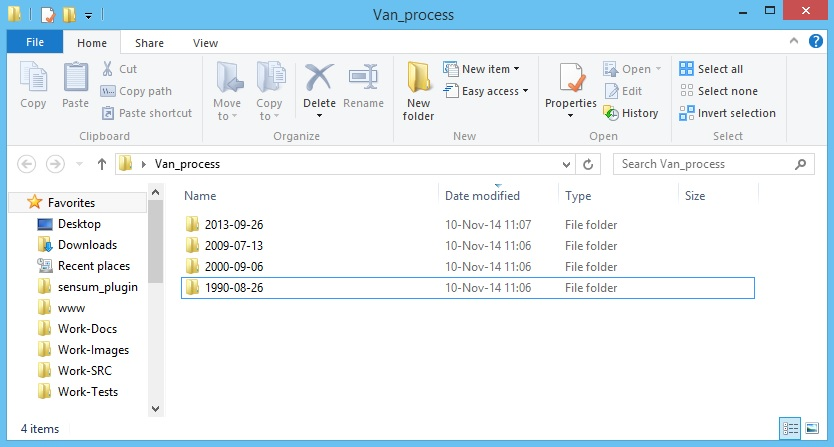
\includegraphics{sat_folder.png}

\end{description}

\item[{\textbf{PARAMETERS}}] \leavevmode\begin{description}
\item[{\emph{sat\_folder}}] \leavevmode
Main folder path

\item[{\emph{segmentation\_name}}] \leavevmode
``Edison'' or ``Meanshift''

\item[{\emph{n\_classes}}] \leavevmode
Number of classes in unsupervised classification

\item[{\emph{--coregistration}}] \leavevmode
Co-Registration option

\item[{\emph{--builtup\_index\_method}}] \leavevmode
Built-up Index method

\item[{\emph{--pca\_index\_method}}] \leavevmode
PCA index method

\item[{\emph{--pca\_classification\_method}}] \leavevmode
PCA classification method

\item[{\emph{--dissimilarity\_method}}] \leavevmode
Dissimilarity method

\item[{\emph{--pca\_ob\_method}}] \leavevmode
PCA object method

\item[{\emph{--restrict\_to\_city SHAPEFILE}}] \leavevmode
Tiling shapefile.

\item[{\emph{--segmentation\_paramaters PARAMETER1 PARAMETER2 PARAMETER3 PARAMETER4}}] \leavevmode\begin{description}
\item[{Edison:}] \leavevmode\begin{itemize}
\item {} 
PARAMETER1: spatial\_radius

\item {} 
PARAMETER2: range\_radius

\item {} 
PARAMETER3: min\_size

\item {} 
PARAMETER4: scale

\end{itemize}

\item[{Meanshift:}] \leavevmode\begin{itemize}
\item {} 
PARAMETER1: spatial\_radius

\item {} 
PARAMETER2: range\_radius

\item {} 
PARAMETER3: threshold

\item {} 
PARAMETER4: max\_iter

\item {} 
PARAMETER5: min\_size

\end{itemize}

\end{description}

\end{description}

\end{description}

\textbf{EXAMPLES}
\begin{quote}

\emph{Unix}

\begin{Verbatim}[frame=single,commandchars=\\\{\}]
\PYGZti{}/.qgis2/python/plugins/sensum\PYGZus{}plugin/scripts/stacksatellite.py \PYGZdq{}\PYGZti{}/Desktop/Work\PYGZhy{}Images/07\PYGZhy{}D\PYGZhy{}Case12\PYGZdq{} \PYGZdq{}Edison\PYGZdq{} \PYGZdq{}5\PYGZdq{}  \PYGZhy{}\PYGZhy{}restrict\PYGZus{}to\PYGZus{}city \PYGZdq{}\PYGZti{}/Desktop/Work\PYGZhy{}Images/07\PYGZhy{}D\PYGZhy{}Case12/Mask\PYGZus{}reclass1\PYGZus{}Identity.shp\PYGZdq{} \PYGZhy{}\PYGZhy{}coregistration \PYGZhy{}\PYGZhy{}dissimilarity\PYGZus{}method \PYGZhy{}\PYGZhy{}segmentation\PYGZus{}paramaters 5 15 100 1
\end{Verbatim}

\emph{MS Windows}

\begin{Verbatim}[frame=single,commandchars=\\\{\}]
C:/Python27/python.exe \PYGZdq{}HOMEPATH\PYGZpc{}/.qgis2/python/plugins/sensum\PYGZus{}plugin/scripts/stacksatellite.py\PYGZdq{} \PYGZdq{}HOMEPATH\PYGZpc{}/Desktop/Work\PYGZhy{}Images/07\PYGZhy{}D\PYGZhy{}Case12\PYGZdq{} \PYGZdq{}Edison\PYGZdq{} \PYGZdq{}5\PYGZdq{}  \PYGZhy{}\PYGZhy{}restrict\PYGZus{}to\PYGZus{}city \PYGZdq{}HOMEPATH\PYGZpc{}/Desktop/Work\PYGZhy{}Images/07\PYGZhy{}D\PYGZhy{}Case12/Mask\PYGZus{}reclass1\PYGZus{}Identity.shp\PYGZdq{} \PYGZhy{}\PYGZhy{}coregistration \PYGZhy{}\PYGZhy{}dissimilarity\PYGZus{}method \PYGZhy{}\PYGZhy{}segmentation\PYGZus{}paramaters 5 15 100 1
\end{Verbatim}
\end{quote}


\subsubsection{Change Detection}
\label{user:change-detection}\begin{description}
\item[{\textbf{SYNOPSIS:}}] \leavevmode
change\_detection.py \emph{main\_folder extraction field {[}--spatial\_filter{]}}

\item[{\textbf{OUTPUT:}}] \leavevmode
Generate a ``change\_detection\_pca.shp'' or ``change\_detection\_dissimilarity.shp'' file as output into the ``main\_folder'' according to the extraction option.

\item[{\textbf{DESCRIPTION:}}] \leavevmode
change\_detection.py is a script designed to detect changes without user supervision. The algorithm works on the results generate by the stack satellite script.
``Change Detection'' algorithm compares built-up extractions (object-based methods) from different dates and filters results in 3 steps:
\begin{enumerate}
\item {} 
count changes through years in order to analyze the results and assign C\_Factor 0 to no changes, C\_Factor 1 to one correct change and from 0.5 to 1 to no possible change or more than 1 change.

\item {} 
time- and continuity-wise change analysis by taking 4-years-span windows to correct sequence with 1 or more possible changes.

\item {} 
applied to undetermined changes coming from step 2, it is designed to process features around the undetermined ones in order to find a spatial similarity with the neighbors.

\end{enumerate}

\item[{\textbf{PARAMATERS}}] \leavevmode\begin{description}
\item[{\emph{main\_folder}}] \leavevmode
``Stack Satellite style'' folder processed by the stacksatellite.py script.

\item[{\emph{extraction}}] \leavevmode
Select ``PCA'' or ``Dissimilarity'' built-up extraction.

\item[{\emph{field}}] \leavevmode
Attribute in the pca\_class or dissimilarity\_class shapefiles related to built-up areas. You have to manually edit just the first feature of the shape by writing the classes related to built-up separated by comma (include screen shot as example).

\end{description}

\end{description}

\textbf{EXAMPLES}
\begin{quote}

\emph{Unix}

\begin{Verbatim}[frame=single,commandchars=\\\{\}]
\PYGZti{}/.qgis2/python/plugins/sensum\PYGZus{}plugin/scripts/change\PYGZus{}detection.py \PYGZdq{}\PYGZti{}/Work\PYGZhy{}Images/Change\PYGZus{}detection\PYGZus{}Izmir\PYGZdq{} \PYGZdq{}PCA\PYGZdq{} \PYGZdq{}UrbanClass\PYGZdq{}
\end{Verbatim}

\emph{MS Windows}

\begin{Verbatim}[frame=single,commandchars=\\\{\}]
C:/Python27/python.exe \PYGZdq{}HOMEPATH\PYGZpc{}/.qgis2/python/plugins/sensum\PYGZus{}plugin/scripts/change\PYGZus{}detection.py\PYGZdq{} \PYGZdq{}HOMEPATH\PYGZpc{}/Desktop/Work\PYGZhy{}Images/Change\PYGZus{}detection\PYGZus{}Izmir\PYGZdq{} \PYGZdq{}PCA\PYGZdq{} \PYGZdq{}UrbanClass\PYGZdq{}
\end{Verbatim}
\end{quote}

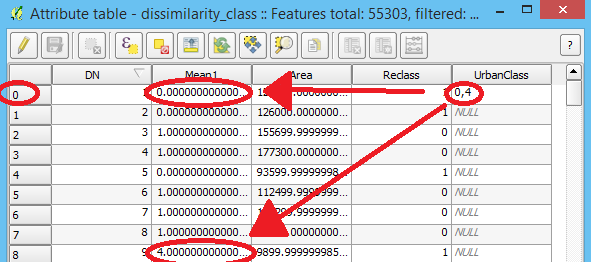
\includegraphics{change_detection.png}


\subsection{High Resolution}
\label{user:high-resolution}

\subsubsection{Footprints}
\label{user:footprints}\begin{description}
\item[{\textbf{SYNOPSIS:}}] \leavevmode
footprints.py \emph{pansharp\_file training\_set training\_attribute output\_shape {[}--classes CLASS1, CLASS2, ...{]} {[}--optimizer\}}

\item[{\textbf{OUTPUT:}}] \leavevmode
Generate a shapefile ({\color{red}\bfseries{}*}.shp) named as the output\_shape parameter.

\item[{\textbf{DESCRIPTION:}}] \leavevmode\begin{description}
\item[{footprints.py is an algorithm developed in order to extract building footprints from supervised classification. Inputs are a pan-sharpened image and a training set shapefile (for the supervised classification). The list of classes related to buildings is also requested. The process is made of 5 steps:}] \leavevmode\begin{enumerate}
\item {} 
Optional OTB Smooth Filter.

\item {} 
OTB supervised classification (Support Vector Machine, SVM).

\item {} 
Conversion of classification output to shapefile.

\item {} 
Masking and filtering of the classes related to buildings.

\item {} 
Morphological filtering.

\end{enumerate}

\end{description}

\item[{\textbf{PARAMETERS}}] \leavevmode\begin{description}
\item[{\emph{pansharp\_file}}] \leavevmode
Pan-sharpened input raster

\item[{\emph{training\_set}}] \leavevmode
Training set as shapefile

\item[{\emph{training\_attribute}}] \leavevmode
Training Field identifier

\item[{\emph{output\_shape}}] \leavevmode
Output shapefile

\item[{\emph{--classes CLASS1, CLASS2, ...}}] \leavevmode
Buildings class selection

\item[{\emph{--optimizer}}] \leavevmode
Enable smooth filter

\end{description}

\end{description}

\textbf{EXAMPLES}
\begin{quote}

\emph{Unix}

\begin{Verbatim}[frame=single,commandchars=\\\{\}]
\PYGZti{}/.qgis2/python/plugins/sensum\PYGZus{}plugin/scripts/footprints.py \PYGZdq{}\PYGZti{}/Desktop/Work\PYGZhy{}Images/Exercises/7/pansharp.tif\PYGZdq{} \PYGZdq{}\PYGZti{}/Desktop/Work\PYGZhy{}Images/Exercises/6/Izmir\PYGZus{}low\PYGZus{}residential\PYGZus{}small\PYGZus{}patches\PYGZus{}footprints\PYGZus{}rpj.shp\PYGZdq{} \PYGZdq{}Class\PYGZdq{} \PYGZdq{}\PYGZti{}/Desktop/Work\PYGZhy{}Tests/building\PYGZus{}extraction.shp\PYGZdq{}  \PYGZhy{}c \PYGZdq{}3\PYGZdq{} \PYGZdq{}1\PYGZdq{}
\end{Verbatim}

\emph{MS Windows}

\begin{Verbatim}[frame=single,commandchars=\\\{\}]
C:/Python27/python.exe \PYGZdq{}HOMEPATH\PYGZpc{}/.qgis2/python/plugins/sensum\PYGZus{}plugin/scripts/footprints.py\PYGZdq{} \PYGZdq{}HOMEPATH\PYGZpc{}/Desktop/Work\PYGZhy{}Images/Exercises/7/pansharp.tif\PYGZdq{} \PYGZdq{}HOMEPATH\PYGZpc{}/Desktop/Work\PYGZhy{}Images/Exercises/6/Izmir\PYGZus{}low\PYGZus{}residential\PYGZus{}small\PYGZus{}patches\PYGZus{}footprints\PYGZus{}rpj.shp\PYGZdq{} \PYGZdq{}Class\PYGZdq{} \PYGZdq{}HOMEPATH\PYGZpc{}/Desktop/Work\PYGZhy{}Tests/building\PYGZus{}extraction.shp\PYGZdq{}  \PYGZhy{}c \PYGZdq{}3\PYGZdq{} \PYGZdq{}1\PYGZdq{}
\end{Verbatim}
\end{quote}


\subsubsection{Density}
\label{user:density}\begin{description}
\item[{\textbf{SYNOPSIS:}}] \leavevmode
density.py \emph{buildingShape radius outputShape}

\item[{\textbf{OUTPUT:}}] \leavevmode
Generate a shapefile ({\color{red}\bfseries{}*}.shp) into outputShape path.

\item[{\textbf{DESCRIPTION:}}] \leavevmode
density.py is a script to compute the building density. It considers a circular window around each feature and calculates how many other features intersect it adding value into ``N\_Building'' row into shapefile. ``Density'' attribute is also computed using \emph{Features Sum Area/Window Area}.

\item[{\textbf{PARAMATERS}}] \leavevmode\begin{description}
\item[{\emph{buildingShape}}] \leavevmode
Building shapefile path

\item[{\emph{radius}}] \leavevmode
Radius of windows

\item[{\emph{outputShape}}] \leavevmode
Output shapefile

\end{description}

\end{description}

\textbf{EXAMPLES}
\begin{quote}

\emph{Unix}

\begin{Verbatim}[frame=single,commandchars=\\\{\}]
\PYGZti{}/.qgis2/python/plugins/sensum\PYGZus{}plugin/scripts/density.py \PYGZdq{}\PYGZti{}/Desktop/Work\PYGZhy{}Tests/building\PYGZus{}extraction.shp\PYGZdq{} \PYGZdq{}10.0\PYGZdq{} \PYGZdq{}\PYGZti{}/Desktop/Work\PYGZhy{}Tests/density.shp\PYGZdq{}
\end{Verbatim}

\emph{MS Windows}

\begin{Verbatim}[frame=single,commandchars=\\\{\}]
C:/Python27/python.exe \PYGZdq{}HOMEPATH\PYGZpc{}/.qgis2/python/plugins/sensum\PYGZus{}plugin/scripts/density.py\PYGZdq{} \PYGZdq{}HOMEPATH\PYGZpc{}/Desktop/Work\PYGZhy{}Tests/building\PYGZus{}extraction.shp\PYGZdq{} \PYGZdq{}10.0\PYGZdq{} \PYGZdq{}HOMEPATH\PYGZpc{}/Desktop/Work\PYGZhy{}Tests/density.shp\PYGZdq{}
\end{Verbatim}
\end{quote}


\subsubsection{Height}
\label{user:height}\begin{description}
\item[{\textbf{SYNOPSIS:}}] \leavevmode
height.py \emph{input\_shadow input\_buildings date output\_shape idfield window\_resize}

\item[{\textbf{OUTPUT:}}] \leavevmode
Generate a shapefile ({\color{red}\bfseries{}*}.shp) into outputShape path.

\item[{\textbf{DESCRIPTION:}}] \leavevmode
height.py is an algorithm designed to estimate the height of buildings from shadows and acquisition date. The result is automatically assigned to related footprints.

\item[{\textbf{PARAMATERS}}] \leavevmode\begin{description}
\item[{\emph{input\_shadow}}] \leavevmode
Shadows shapefile path

\item[{\emph{input\_buildings}}] \leavevmode
Building shapefile path

\item[{\emph{date}}] \leavevmode
Acquisition date (hour in EDT)

\item[{\emph{output\_shape}}] \leavevmode
Output shapefile

\item[{\emph{idfield}}] \leavevmode
Shadow ID field

\item[{\emph{window\_resize}}] \leavevmode
Searching window radius

\end{description}

\end{description}

\textbf{EXAMPLES}
\begin{quote}

\emph{Unix}

\begin{Verbatim}[frame=single,commandchars=\\\{\}]
\PYGZti{}/.qgis2/python/plugins/sensum\PYGZus{}plugin/scripts/height.py \PYGZdq{}\PYGZti{}/Desktop/Work\PYGZhy{}Tests/building\PYGZus{}extraction.shp\PYGZdq{} \PYGZdq{}\PYGZti{}/Desktop/Work\PYGZhy{}Tests/building\PYGZus{}shadows.shp\PYGZdq{} \PYGZdq{}2007/1/17 15:34:00\PYGZdq{} \PYGZdq{}height.shp\PYGZdq{} \PYGZdq{}ID\PYGZdq{} \PYGZdq{}1.0\PYGZdq{}
\end{Verbatim}

\emph{MS Windows}

\begin{Verbatim}[frame=single,commandchars=\\\{\}]
C:/Python27/python.exe \PYGZdq{}HOMEPATH\PYGZpc{}/.qgis2/python/plugins/sensum\PYGZus{}plugin/scripts/height.py\PYGZdq{} \PYGZdq{}HOMEPATH\PYGZpc{}/Desktop/Work\PYGZhy{}Tests/building\PYGZus{}extraction.shp\PYGZdq{} \PYGZdq{}HOMEPATH\PYGZpc{}/Desktop/Work\PYGZhy{}Tests/building\PYGZus{}shadows.shp\PYGZdq{} \PYGZdq{}2007/1/17 15:34:00\PYGZdq{} \PYGZdq{}height.shp\PYGZdq{} \PYGZdq{}ID\PYGZdq{} \PYGZdq{}1.0\PYGZdq{}
\end{Verbatim}
\end{quote}


\subsubsection{Regularity}
\label{user:regularity}\begin{description}
\item[{\textbf{SYNOPSIS:}}] \leavevmode
regularity.py \emph{input\_buildings output\_shape}

\item[{\textbf{OUTPUT:}}] \leavevmode
Generate a shapefile ({\color{red}\bfseries{}*}.shp) into outputShape path.

\item[{\textbf{DESCRIPTION:}}] \leavevmode
regularity.py can be used to determine the regularity and alignment of buildings. A polygon is considered regular when the ratio between the two main directions is less than 4.

\item[{\textbf{PARAMATERS}}] \leavevmode\begin{description}
\item[{\emph{input\_buildings}}] \leavevmode
Input buildings shapefile path

\item[{\emph{output\_shape}}] \leavevmode
Output shapefile

\end{description}

\end{description}

\textbf{EXAMPLES}
\begin{quote}

\emph{Unix}

\begin{Verbatim}[frame=single,commandchars=\\\{\}]
\PYGZti{}/.qgis2/python/plugins/sensum\PYGZus{}plugin/scripts/regularity.py \PYGZdq{}\PYGZti{}/Desktop/Work\PYGZhy{}Tests/building\PYGZus{}extraction.shp\PYGZdq{} \PYGZdq{}\PYGZti{}/Desktop/Work\PYGZhy{}Tests/regularity.shp\PYGZdq{}
\end{Verbatim}

\emph{MS Windows}

\begin{Verbatim}[frame=single,commandchars=\\\{\}]
C:/Python27/python.exe \PYGZdq{}HOMEPATH\PYGZpc{}/.qgis2/python/plugins/sensum\PYGZus{}plugin/scripts/regularity.py\PYGZdq{} \PYGZdq{}HOMEPATH\PYGZpc{}/Desktop/Work\PYGZhy{}Tests/building\PYGZus{}extraction.shp\PYGZdq{} \PYGZdq{}HOMEPATH\PYGZpc{}/Desktop/Work\PYGZhy{}Tests/regularity.shp\PYGZdq{}
\end{Verbatim}
\end{quote}


\subsection{Test Features}
\label{user:test-features}\begin{description}
\item[{\textbf{SYNOPSIS:}}] \leavevmode
test\_features.py \emph{input\_file segmentation\_shape output\_shape field {[}--max\_br{]} {[}--mean{]} {[}--min\_br{]} {[}--mode{]} {[}--ndvi\_std{]} {[}--ndvi\_mean{]} {[}--std{]} {[}--weigh\_br{]} {[}--ASM{]} {[}--contrast{]} {[}--correlation{]} {[}--dissimilarity{]} {[}--energy{]} {[}--homogeneity{]} {[}--multi{]}}

\item[{\textbf{OUTPUT:}}] \leavevmode
A shapefile is generated in output\_shape path

\item[{\textbf{DESCRIPTION:}}] \leavevmode
test\_features.py is a script made to compute a set of features related to segments. Statistics are calculated based on the input raster file using a segmentation shapefile as mask. Computed features are appended as attribute to the shapefile.

\item[{\textbf{PARAMATERS}}] \leavevmode\begin{description}
\item[{\emph{input\_file}}] \leavevmode
Input raster file

\item[{\emph{segmentation\_shape}}] \leavevmode
Segmentation shape mask

\item[{\emph{output\_shape}}] \leavevmode
Output shapefile

\item[{\emph{field}}] \leavevmode
Identifier shapefile ID

\item[{\emph{--max\_br}}] \leavevmode
Maximum BR

\item[{\emph{--mean}}] \leavevmode
Mean

\item[{\emph{--min\_br}}] \leavevmode
Minimun BR

\item[{\emph{--mode}}] \leavevmode
Mode

\item[{\emph{--ndvi\_std}}] \leavevmode
NDVI Standard Deviation

\item[{\emph{--ndvi\_mean}}] \leavevmode
NDVI Mean

\item[{\emph{--std}}] \leavevmode
Standard Deviation

\item[{\emph{--weigh\_br}}] \leavevmode
Weight BR

\item[{\emph{--ASM}}] \leavevmode
ASM

\item[{\emph{--contrast}}] \leavevmode
Contrast

\item[{\emph{--correlation}}] \leavevmode
Correlation

\item[{\emph{--energy}}] \leavevmode
Energy

\item[{\emph{--homogeneity}}] \leavevmode
Homogeneity

\item[{\emph{--multi}}] \leavevmode
Active multiprocess option (hight CPU usage)

\end{description}

\end{description}

\textbf{EXAMPLES}
\begin{quote}

\emph{Unix}

\begin{Verbatim}[frame=single,commandchars=\\\{\}]
\PYGZti{}/.qgis2/python/plugins/sensum\PYGZus{}plugin/scripts/test\PYGZus{}features.py \PYGZdq{}\PYGZti{}/Desktop/Work\PYGZhy{}Tests/input.tiff\PYGZdq{} \PYGZdq{}\PYGZti{}/Desktop/Work\PYGZhy{}Tests/building\PYGZus{}extraction.shp\PYGZdq{} \PYGZdq{}\PYGZti{}/Desktop/Work\PYGZhy{}Tests/features\PYGZus{}calculation.shp\PYGZdq{} \PYGZdq{}DN\PYGZdq{} \PYGZhy{}\PYGZhy{}max\PYGZus{}br \PYGZhy{}\PYGZhy{}mode \PYGZhy{}\PYGZhy{}contrast \PYGZhy{}\PYGZhy{}energy
\end{Verbatim}

\emph{MS Windows}

\begin{Verbatim}[frame=single,commandchars=\\\{\}]
C:/Python27/python.exe \PYGZdq{}HOMEPATH\PYGZpc{}/.qgis2/python/plugins/sensum\PYGZus{}plugin/scripts/test\PYGZus{}features.py\PYGZdq{} \PYGZdq{}HOMEPATH\PYGZpc{}/Desktop/Work\PYGZhy{}Tests/input.tiff\PYGZdq{} \PYGZdq{}HOMEPATH\PYGZpc{}/Desktop/Work\PYGZhy{}Tests/building\PYGZus{}extraction.shp\PYGZdq{} \PYGZdq{}HOMEPATH\PYGZpc{}/Desktop/Work\PYGZhy{}Tests/features\PYGZus{}calculation.shp\PYGZdq{} \PYGZdq{}DN\PYGZdq{} \PYGZhy{}\PYGZhy{}max\PYGZus{}br \PYGZhy{}\PYGZhy{}mode \PYGZhy{}\PYGZhy{}contrast \PYGZhy{}\PYGZhy{}energy
\end{Verbatim}
\end{quote}


\chapter{The Developer's Guide}
\label{index:the-developer-s-guide}

\section{The Developer's Guide}
\label{lib:the-developer-s-guide}\label{lib::doc}

\subsection{Introduction}
\label{lib:introduction}\begin{description}
\item[{\textbf{General Knowledge}}] \leavevmode
Sensum Earth Observation Tools are written in Python. They make use of Gdal library to read and write rasters files as arrays, handled by Scipy, Numpy, Python math and OpenCV libraries.
OGR is used to read, write and handle vector files. OTB and skimage are used for classification and segmentation algorithms. The Plugin UI is written in PyQT using the qgis.core library to interact with QGIS interface.

\item[{\textbf{Structure}}] \leavevmode
Sensum Library is composed by modules divided according to their scope. To import a Sensum module you have to import the config.py script first in order to automatically set all the necessary variables and configuration settings:

\begin{Verbatim}[frame=single,commandchars=\\\{\}]
\PYG{k+kn}{import} \PYG{n+nn}{config}
\end{Verbatim}

You can import a sensum library module with the following line:

\begin{Verbatim}[frame=single,commandchars=\\\{\}]
\PYG{k+kn}{from} \PYG{n+nn}{sensum\PYGZus{}library.MODULE\PYGZus{}NAME} \PYG{k+kn}{import} \PYG{o}{*}
\end{Verbatim}

\end{description}


\subsection{Conversion, Features}
\label{lib:conversion-features}\begin{description}
\item[{\textbf{Conventions}}] \leavevmode\begin{description}
\item[{This is the main module to read/write and handle rasters. It is composed by a set of functions with a set of convenction:}] \leavevmode\begin{itemize}
\item {} 
0 value is used to set defaults value in a lot of functions parameters.

\item {} 
\emph{band\_list}: is a N-D list of matrices containing pixel values read with gdal ReadAsArray method, where N = number of bands

\item {} 
\emph{input/output\_raster}: path of raster file

\item {} 
\emph{input/output\_shape}: path of vector file

\end{itemize}

\end{description}

\item[{\textbf{Main Functions}}] \leavevmode
Main functions are read\_image , write\_image used to read and write rasters files.

\end{description}


\subsection{Classification, Segmentation}
\label{lib:classification-segmentation}
Classification and segmentation modules include functions to define hubs between python and OTB and skimage in order to take advantage of classification and segmentation algorithms. In some scripts or plugin parts a system call for external compiled OTB executable is included in order to get the process progress bar. This is achieved using the executeOtb function:

\begin{Verbatim}[frame=single,commandchars=\\\{\},numbers=left,firstnumber=1,stepnumber=1]
    \PYG{k}{if} \PYG{n}{os}\PYG{o}{.}\PYG{n}{name} \PYG{o}{!=} \PYG{l+s}{\PYGZdq{}}\PYG{l+s}{posix}\PYG{l+s}{\PYGZdq{}}\PYG{p}{:}
        \PYG{n}{bit} \PYG{o}{=} \PYG{p}{(}\PYG{l+s}{\PYGZdq{}}\PYG{l+s}{64}\PYG{l+s}{\PYGZdq{}} \PYG{k}{if} \PYG{n}{os}\PYG{o}{.}\PYG{n}{path}\PYG{o}{.}\PYG{n}{isdir}\PYG{p}{(}\PYG{l+s}{\PYGZdq{}}\PYG{l+s}{C:/OSGeo4W64}\PYG{l+s}{\PYGZdq{}}\PYG{p}{)} \PYG{k}{else} \PYG{l+s}{\PYGZdq{}}\PYG{l+s}{\PYGZdq{}}\PYG{p}{)}
        \PYG{n}{osgeopath} \PYG{o}{=} \PYG{l+s}{\PYGZdq{}}\PYG{l+s}{C:/OSGeo4W\PYGZob{}\PYGZcb{}/bin/}\PYG{l+s}{\PYGZdq{}}\PYG{o}{.}\PYG{n}{format}\PYG{p}{(}\PYG{n}{bit}\PYG{p}{)}
        \PYG{n}{command} \PYG{o}{=} \PYG{n}{osgeopath} \PYG{o}{+} \PYG{n}{command}
    \PYG{c}{\PYGZsh{}QMessageBox.information(None, \PYGZdq{}Info\PYGZdq{}, command)    }
    \PYG{n}{proc} \PYG{o}{=} \PYG{n}{subprocess}\PYG{o}{.}\PYG{n}{Popen}\PYG{p}{(}
        \PYG{n}{command}\PYG{p}{,}
        \PYG{n}{shell}\PYG{o}{=}\PYG{n+nb+bp}{True}\PYG{p}{,}
        \PYG{n}{stdout}\PYG{o}{=}\PYG{n}{subprocess}\PYG{o}{.}\PYG{n}{PIPE}\PYG{p}{,}
        \PYG{n}{stdin}\PYG{o}{=}\PYG{n}{subprocess}\PYG{o}{.}\PYG{n}{PIPE}\PYG{p}{,}
        \PYG{n}{stderr}\PYG{o}{=}\PYG{n}{subprocess}\PYG{o}{.}\PYG{n}{STDOUT}\PYG{p}{,}
        \PYG{n}{universal\PYGZus{}newlines}\PYG{o}{=}\PYG{n+nb+bp}{True}\PYG{p}{,}
        \PYG{p}{)}\PYG{o}{.}\PYG{n}{stdout}
    \PYG{k}{for} \PYG{n}{line} \PYG{o+ow}{in} \PYG{n+nb}{iter}\PYG{p}{(}\PYG{n}{proc}\PYG{o}{.}\PYG{n}{readline}\PYG{p}{,} \PYG{l+s}{\PYGZsq{}}\PYG{l+s}{\PYGZsq{}}\PYG{p}{)}\PYG{p}{:}
        \PYG{k}{if} \PYG{l+s}{\PYGZsq{}}\PYG{l+s}{[*}\PYG{l+s}{\PYGZsq{}} \PYG{o+ow}{in} \PYG{n}{line}\PYG{p}{:}
            \PYG{n}{idx} \PYG{o}{=} \PYG{n}{line}\PYG{o}{.}\PYG{n}{find}\PYG{p}{(}\PYG{l+s}{\PYGZsq{}}\PYG{l+s}{[*}\PYG{l+s}{\PYGZsq{}}\PYG{p}{)}
            \PYG{n}{perc} \PYG{o}{=} \PYG{n+nb}{int}\PYG{p}{(}\PYG{n}{line}\PYG{p}{[}\PYG{n}{idx} \PYG{o}{\PYGZhy{}} \PYG{l+m+mi}{4}\PYG{p}{:}\PYG{n}{idx} \PYG{o}{\PYGZhy{}} \PYG{l+m+mi}{2}\PYG{p}{]}\PYG{o}{.}\PYG{n}{strip}\PYG{p}{(}\PYG{l+s}{\PYGZsq{}}\PYG{l+s}{ }\PYG{l+s}{\PYGZsq{}}\PYG{p}{)}\PYG{p}{)}
            \PYG{k}{if} \PYG{n}{perc} \PYG{o}{!=} \PYG{l+m+mi}{0} \PYG{o+ow}{and} \PYG{n}{progress}\PYG{p}{:}
                \PYG{n}{progress}\PYG{o}{.}\PYG{n}{progressBar}\PYG{o}{.}\PYG{n}{setValue}\PYG{p}{(}\PYG{n}{perc}\PYG{p}{)}
                \PYG{n}{progress}\PYG{o}{.}\PYG{n}{label\PYGZus{}title}\PYG{o}{.}\PYG{n}{setText}\PYG{p}{(}\PYG{n}{label}\PYG{p}{)}
        \PYG{n}{QtGui}\PYG{o}{.}\PYG{n}{qApp}\PYG{o}{.}\PYG{n}{processEvents}\PYG{p}{(}\PYG{p}{)}
\end{Verbatim}


\subsection{Preprocess, Secondary Indicators}
\label{lib:preprocess-secondary-indicators}
Contains a series of scripts and tools functions.


\subsection{Multi}
\label{lib:multi}
\textbf{Intro}
Multiprocess module is dedicated to multiprocess application. Python provides a powerful built-in multiprocess library; the Sensum multiprocess module uses this library to implement multiprocess applications through a container Class. This solution was specifically designed to provide clean and easy implementation also for non-expert developers.

\textbf{Description}
\begin{quote}

Multi() class defines N concurrent processes with N = number of CPU core * 2.
\end{quote}
\begin{description}
\item[{\textbf{Example}}] \leavevmode
We want to implement with multiprocess a simple function for get the sum between a number and his double within a range from 0 to 100:

\begin{Verbatim}[frame=single,commandchars=\\\{\}]
\PYG{k}{def} \PYG{n+nf}{task}\PYG{p}{(}\PYG{n}{a}\PYG{p}{)}\PYG{p}{:}
    \PYG{k}{return} \PYG{n}{a}\PYG{o}{*}\PYG{l+m+mi}{2}\PYG{o}{+}\PYG{n}{a}

\PYG{k}{for} \PYG{n}{i} \PYG{o+ow}{in} \PYG{n+nb}{range}\PYG{p}{(}\PYG{l+m+mi}{101}\PYG{p}{)}\PYG{p}{:}
    \PYG{k}{print} \PYG{n}{task}\PYG{p}{(}\PYG{n}{i}\PYG{p}{)}
\end{Verbatim}

To implement task() as multiprocess we need to reclass it as a callable Class:

\begin{Verbatim}[frame=single,commandchars=\\\{\}]
\PYG{k}{class} \PYG{n+nc}{Task}\PYG{p}{(}\PYG{n+nb}{object}\PYG{p}{)}\PYG{p}{:}
    \PYG{k}{def} \PYG{n+nf}{\PYGZus{}\PYGZus{}init\PYGZus{}\PYGZus{}}\PYG{p}{(}\PYG{n+nb+bp}{self}\PYG{p}{,} \PYG{n}{a}\PYG{p}{)}\PYG{p}{:}
        \PYG{n+nb+bp}{self}\PYG{o}{.}\PYG{n}{index} \PYG{o}{=} \PYG{n}{a}
        \PYG{n+nb+bp}{self}\PYG{o}{.}\PYG{n}{a} \PYG{o}{=} \PYG{n}{a}
    \PYG{k}{def} \PYG{n+nf}{\PYGZus{}\PYGZus{}call\PYGZus{}\PYGZus{}}\PYG{p}{(}\PYG{n+nb+bp}{self}\PYG{p}{)}\PYG{p}{:}
        \PYG{k}{return} \PYG{n+nb+bp}{self}\PYG{o}{.}\PYG{n}{index}\PYG{p}{,}\PYG{n+nb+bp}{self}\PYG{o}{.}\PYG{n}{a}\PYG{o}{*}\PYG{l+m+mi}{2}\PYG{o}{+}\PYG{n+nb+bp}{self}\PYG{o}{.}\PYG{n}{a}
\end{Verbatim}

Unlike function declaration, we need to return also the index since results will not be sorted because multiprocess execution is asynchronous. Now we can implement Task() into the for statement:

\begin{Verbatim}[frame=single,commandchars=\\\{\}]
\PYG{k+kn}{from} \PYG{n+nn}{sensum\PYGZus{}library.multiprocess} \PYG{k+kn}{import} \PYG{o}{*}
\PYG{n}{MyMulti} \PYG{o}{=} \PYG{n}{Multi}\PYG{p}{(}\PYG{p}{)}
\PYG{k}{for} \PYG{n}{i} \PYG{o+ow}{in} \PYG{n+nb}{xrange}\PYG{p}{(}\PYG{l+m+mi}{101}\PYG{p}{)}\PYG{p}{:}
    \PYG{n}{MyMulti}\PYG{o}{.}\PYG{n}{put}\PYG{p}{(}\PYG{n}{Task}\PYG{p}{(}\PYG{n}{i}\PYG{p}{)}\PYG{p}{)}
\PYG{n}{MyMulti}\PYG{o}{.}\PYG{n}{kill}\PYG{p}{(}\PYG{p}{)}
\end{Verbatim}

Use the following lines to get the results, sort and print them:

\begin{Verbatim}[frame=single,commandchars=\\\{\}]
\PYG{n}{results} \PYG{o}{=} \PYG{p}{[} \PYG{n}{MyMulti}\PYG{o}{.}\PYG{n}{result}\PYG{p}{(}\PYG{p}{)} \PYG{k}{for} \PYG{n}{i} \PYG{o+ow}{in} \PYG{n+nb}{xrange}\PYG{p}{(}\PYG{l+m+mi}{101}\PYG{p}{)} \PYG{p}{]}
\PYG{n}{results}\PYG{o}{.}\PYG{n}{sort}\PYG{p}{(}\PYG{p}{)}
\PYG{n}{results} \PYG{o}{=} \PYG{p}{[} \PYG{n}{data} \PYG{k}{for} \PYG{n}{i}\PYG{p}{,}\PYG{n}{data} \PYG{o+ow}{in} \PYG{n}{results} \PYG{p}{]}

\PYG{k}{for} \PYG{n}{data} \PYG{o+ow}{in} \PYG{n}{results}\PYG{p}{:}
    \PYG{k}{print} \PYG{n}{data}
\end{Verbatim}

\end{description}

Following the complete code example:

\begin{Verbatim}[frame=single,commandchars=\\\{\},numbers=left,firstnumber=1,stepnumber=1]
\PYG{k}{if} \PYG{n}{\PYGZus{}\PYGZus{}name\PYGZus{}\PYGZus{}} \PYG{o}{==} \PYG{l+s}{\PYGZsq{}}\PYG{l+s}{\PYGZus{}\PYGZus{}main\PYGZus{}\PYGZus{}}\PYG{l+s}{\PYGZsq{}}\PYG{p}{:}

    \PYG{k}{class} \PYG{n+nc}{Task}\PYG{p}{(}\PYG{n+nb}{object}\PYG{p}{)}\PYG{p}{:}
        \PYG{k}{def} \PYG{n+nf}{\PYGZus{}\PYGZus{}init\PYGZus{}\PYGZus{}}\PYG{p}{(}\PYG{n+nb+bp}{self}\PYG{p}{,} \PYG{n}{a}\PYG{p}{,} \PYG{n}{b}\PYG{p}{)}\PYG{p}{:}
            \PYG{n+nb+bp}{self}\PYG{o}{.}\PYG{n}{a} \PYG{o}{=} \PYG{n}{a}
            \PYG{n+nb+bp}{self}\PYG{o}{.}\PYG{n}{b} \PYG{o}{=} \PYG{n}{b}
        \PYG{k}{def} \PYG{n+nf}{\PYGZus{}\PYGZus{}call\PYGZus{}\PYGZus{}}\PYG{p}{(}\PYG{n+nb+bp}{self}\PYG{p}{)}\PYG{p}{:}
            \PYG{n}{time}\PYG{o}{.}\PYG{n}{sleep}\PYG{p}{(}\PYG{l+m+mi}{1}\PYG{p}{)} \PYG{c}{\PYGZsh{} pretend to take some time to do the work}
            \PYG{k}{return} \PYG{n+nb+bp}{self}\PYG{o}{.}\PYG{n}{a}\PYG{o}{*}\PYG{n+nb+bp}{self}\PYG{o}{.}\PYG{n}{b}
        \PYG{k}{def} \PYG{n+nf}{\PYGZus{}\PYGZus{}str\PYGZus{}\PYGZus{}}\PYG{p}{(}\PYG{n+nb+bp}{self}\PYG{p}{)}\PYG{p}{:}
            \PYG{k}{return} \PYG{n+nb}{str}\PYG{p}{(}\PYG{n+nb+bp}{self}\PYG{o}{.}\PYG{n}{a}\PYG{o}{*}\PYG{n+nb+bp}{self}\PYG{o}{.}\PYG{n}{b}\PYG{p}{)}

    \PYG{k+kn}{import} \PYG{n+nn}{sys}
    \PYG{n}{sys}\PYG{o}{.}\PYG{n}{path}\PYG{o}{.}\PYG{n}{append}\PYG{p}{(}\PYG{l+s}{\PYGZsq{}}\PYG{l+s}{C:/OSGeo4W/apps/Python27/Lib/site\PYGZhy{}packages}\PYG{l+s}{\PYGZsq{}}\PYG{p}{)}

    \PYG{n}{new\PYGZus{}proc} \PYG{o}{=} \PYG{n}{Multi}\PYG{p}{(}\PYG{p}{)}

    \PYG{n}{n\PYGZus{}jobs} \PYG{o}{=} \PYG{l+m+mi}{10}

    \PYG{k}{for} \PYG{n}{i} \PYG{o+ow}{in} \PYG{n+nb}{xrange}\PYG{p}{(}\PYG{n}{n\PYGZus{}jobs}\PYG{p}{)}\PYG{p}{:}
\end{Verbatim}


\subsection{Scripts}
\label{lib:scripts}
For more info about the script system click here

\textbf{Progress Bar}

This is a class used to draw a textual process bar compatible with plugin parser:

\begin{Verbatim}[frame=single,commandchars=\\\{\},numbers=left,firstnumber=1,stepnumber=1]
\PYG{k}{class} \PYG{n+nc}{Bar}\PYG{p}{(}\PYG{n+nb}{object}\PYG{p}{)}\PYG{p}{:}

    \PYG{k}{def} \PYG{n+nf}{\PYGZus{}\PYGZus{}init\PYGZus{}\PYGZus{}}\PYG{p}{(}\PYG{n+nb+bp}{self}\PYG{p}{,} \PYG{n+nb}{max}\PYG{p}{,} \PYG{n}{status}\PYG{o}{=}\PYG{l+s}{\PYGZdq{}}\PYG{l+s}{\PYGZdq{}}\PYG{p}{)}\PYG{p}{:}

        \PYG{n+nb+bp}{self}\PYG{o}{.}\PYG{n}{status} \PYG{o}{=} \PYG{n}{status}
        \PYG{n+nb+bp}{self}\PYG{o}{.}\PYG{n}{max} \PYG{o}{=} \PYG{n+nb}{max}
        \PYG{n+nb+bp}{self}\PYG{o}{.}\PYG{n}{dimension} \PYG{o}{=} \PYG{l+m+mi}{100}
        \PYG{n+nb+bp}{self}\PYG{o}{.}\PYG{n}{\PYGZus{}current} \PYG{o}{=} \PYG{l+m+mi}{0}
        \PYG{n+nb+bp}{self}\PYG{p}{(}\PYG{n+nb+bp}{self}\PYG{o}{.}\PYG{n}{\PYGZus{}current}\PYG{p}{)}

    \PYG{k}{def} \PYG{n+nf}{\PYGZus{}\PYGZus{}call\PYGZus{}\PYGZus{}}\PYG{p}{(}\PYG{n+nb+bp}{self}\PYG{p}{,} \PYG{n}{value}\PYG{p}{,} \PYG{n}{status}\PYG{o}{=}\PYG{n+nb+bp}{None}\PYG{p}{)}\PYG{p}{:}

        \PYG{n}{value} \PYG{o}{=} \PYG{n+nb}{float}\PYG{p}{(}\PYG{n}{value}\PYG{p}{)}
        \PYG{n}{\PYGZus{}current} \PYG{o}{=} \PYG{n+nb}{int}\PYG{p}{(}\PYG{n}{value} \PYG{o}{/} \PYG{n+nb+bp}{self}\PYG{o}{.}\PYG{n}{max} \PYG{o}{*} \PYG{n+nb+bp}{self}\PYG{o}{.}\PYG{n}{dimension}\PYG{p}{)}
        \PYG{k}{if} \PYG{n}{status}\PYG{p}{:}
            \PYG{n+nb+bp}{self}\PYG{o}{.}\PYG{n}{status} \PYG{o}{=} \PYG{n}{status}
        \PYG{k}{if} \PYG{n}{\PYGZus{}current} \PYG{o}{\PYGZgt{}} \PYG{n+nb+bp}{self}\PYG{o}{.}\PYG{n}{\PYGZus{}current}\PYG{p}{:}
            \PYG{n}{wildcards} \PYG{o}{=} \PYG{n}{spaces} \PYG{o}{=} \PYG{l+s}{\PYGZdq{}}\PYG{l+s}{\PYGZdq{}}
            \PYG{k}{for} \PYG{n}{\PYGZus{}} \PYG{o+ow}{in} \PYG{n+nb}{range}\PYG{p}{(}\PYG{n}{\PYGZus{}current}\PYG{p}{)}\PYG{p}{:} \PYG{n}{wildcards} \PYG{o}{=} \PYG{n}{wildcards} \PYG{o}{+} \PYG{l+s}{\PYGZdq{}}\PYG{l+s}{*}\PYG{l+s}{\PYGZdq{}}
            \PYG{k}{for} \PYG{n}{\PYGZus{}} \PYG{o+ow}{in} \PYG{n+nb}{range}\PYG{p}{(}\PYG{n+nb+bp}{self}\PYG{o}{.}\PYG{n}{dimension}\PYG{o}{\PYGZhy{}}\PYG{n}{\PYGZus{}current}\PYG{p}{)}\PYG{p}{:} \PYG{n}{wildcards} \PYG{o}{=} \PYG{n}{wildcards} \PYG{o}{+} \PYG{l+s}{\PYGZdq{}}\PYG{l+s}{ }\PYG{l+s}{\PYGZdq{}}
            \PYG{n}{bar} \PYG{o}{=} \PYG{l+s}{\PYGZdq{}}\PYG{l+s+se}{\PYGZbs{}r}\PYG{l+s}{STATUS: }\PYG{l+s}{\PYGZdq{}} \PYG{o}{+} \PYG{n+nb+bp}{self}\PYG{o}{.}\PYG{n}{status} \PYG{o}{+} \PYG{l+s}{\PYGZdq{}}\PYG{l+s}{ [}\PYG{l+s}{\PYGZdq{}} \PYG{o}{+} \PYG{n}{wildcards} \PYG{o}{+} \PYG{n}{spaces} \PYG{o}{+} \PYG{l+s}{\PYGZdq{}}\PYG{l+s}{]}\PYG{l+s}{\PYGZdq{}}
\end{Verbatim}

Use is simple:

\begin{Verbatim}[frame=single,commandchars=\\\{\}]
n\PYGZus{}list = range(100,200)
status = Bar(len(n\PYGZus{}list),\PYGZdq{}Power N\PYGZdq{})
for i,value in n\PYGZus{}list
    status(i)
    print value*value
\end{Verbatim}


\subsection{Plugin}
\label{lib:plugin}\begin{description}
\item[{\textbf{PyQGIS Developer Cookbook}}] \leavevmode
For more details go to \href{http://docs.qgis.org/2.0/en/docs/pyqgis\_developer\_cookbook/}{http://docs.qgis.org/2.0/en/docs/pyqgis\_developer\_cookbook/}

\end{description}

\textbf{Call Scripts}
To call scripts, the Sensum Plugin uses a function also able to parse the textual progress bar generated by the script:

\begin{Verbatim}[frame=single,commandchars=\\\{\},numbers=left,firstnumber=1,stepnumber=1]
\PYG{k}{def} \PYG{n+nf}{executeScript}\PYG{p}{(}\PYG{n}{command}\PYG{p}{,} \PYG{n}{progress}\PYG{o}{=}\PYG{n+nb+bp}{None}\PYG{p}{,}\PYG{n}{noerror}\PYG{o}{=}\PYG{n+nb+bp}{True}\PYG{p}{)}\PYG{p}{:}
    \PYG{k}{if} \PYG{n}{os}\PYG{o}{.}\PYG{n}{name} \PYG{o}{!=} \PYG{l+s}{\PYGZdq{}}\PYG{l+s}{posix}\PYG{l+s}{\PYGZdq{}} \PYG{o+ow}{and} \PYG{n}{noerror}\PYG{p}{:}
        \PYG{c}{\PYGZsh{} Found at http://stackoverflow.com/questions/5069224/handling\PYGZhy{}subprocess\PYGZhy{}crash\PYGZhy{}in\PYGZhy{}windows}
        \PYG{c}{\PYGZsh{} Don\PYGZsq{}t display the Windows GPF dialog if the invoked program dies.}
        \PYG{c}{\PYGZsh{} See comp.os.ms\PYGZhy{}windows.programmer.win32}
        \PYG{c}{\PYGZsh{} How to suppress crash notification dialog?, Jan 14,2004 \PYGZhy{}}
        \PYG{c}{\PYGZsh{} Raymond Chen\PYGZsq{}s response [1]}

        \PYG{k+kn}{import} \PYG{n+nn}{ctypes}
        \PYG{n}{SEM\PYGZus{}NOGPFAULTERRORBOX} \PYG{o}{=} \PYG{l+m+mh}{0x0002} \PYG{c}{\PYGZsh{} From MSDN}
        \PYG{n}{ctypes}\PYG{o}{.}\PYG{n}{windll}\PYG{o}{.}\PYG{n}{kernel32}\PYG{o}{.}\PYG{n}{SetErrorMode}\PYG{p}{(}\PYG{n}{SEM\PYGZus{}NOGPFAULTERRORBOX}\PYG{p}{)}\PYG{p}{;}
        \PYG{n}{subprocess\PYGZus{}flags} \PYG{o}{=} \PYG{l+m+mh}{0x8000000} \PYG{c}{\PYGZsh{}win32con.CREATE\PYGZus{}NO\PYGZus{}WINDOW?}
    \PYG{k}{else}\PYG{p}{:}
        \PYG{n}{subprocess\PYGZus{}flags} \PYG{o}{=} \PYG{l+m+mi}{0}

    \PYG{n}{command} \PYG{o}{=} \PYG{p}{(}\PYG{n}{os}\PYG{o}{.}\PYG{n}{path}\PYG{o}{.}\PYG{n}{dirname}\PYG{p}{(}\PYG{n}{os}\PYG{o}{.}\PYG{n}{path}\PYG{o}{.}\PYG{n}{abspath}\PYG{p}{(}\PYG{n}{\PYGZus{}\PYGZus{}file\PYGZus{}\PYGZus{}}\PYG{p}{)}\PYG{p}{)}\PYG{o}{+}\PYG{n}{command} \PYG{k}{if} \PYG{n}{os}\PYG{o}{.}\PYG{n}{name} \PYG{o}{==} \PYG{l+s}{\PYGZdq{}}\PYG{l+s}{posix}\PYG{l+s}{\PYGZdq{}} \PYG{k}{else} \PYG{l+s}{\PYGZsq{}}\PYG{l+s}{C:/Python27/python.exe }\PYG{l+s}{\PYGZdq{}}\PYG{l+s}{\PYGZsq{}}\PYG{o}{+}\PYG{n}{os}\PYG{o}{.}\PYG{n}{path}\PYG{o}{.}\PYG{n}{dirname}\PYG{p}{(}\PYG{n}{os}\PYG{o}{.}\PYG{n}{path}\PYG{o}{.}\PYG{n}{abspath}\PYG{p}{(}\PYG{n}{\PYGZus{}\PYGZus{}file\PYGZus{}\PYGZus{}}\PYG{p}{)}\PYG{p}{)}\PYG{o}{+}\PYG{n}{command}\PYG{p}{)}
    \PYG{n}{QMessageBox}\PYG{o}{.}\PYG{n}{information}\PYG{p}{(}\PYG{n+nb+bp}{None}\PYG{p}{,} \PYG{l+s}{\PYGZdq{}}\PYG{l+s}{Info}\PYG{l+s}{\PYGZdq{}}\PYG{p}{,} \PYG{n}{command}\PYG{p}{)}
    \PYG{n}{proc} \PYG{o}{=} \PYG{n}{subprocess}\PYG{o}{.}\PYG{n}{Popen}\PYG{p}{(}
        \PYG{n}{command}\PYG{p}{,}
        \PYG{n}{shell}\PYG{o}{=}\PYG{n+nb+bp}{True}\PYG{p}{,}
        \PYG{n}{stdout}\PYG{o}{=}\PYG{n}{subprocess}\PYG{o}{.}\PYG{n}{PIPE}\PYG{p}{,}
        \PYG{n}{stdin}\PYG{o}{=}\PYG{n}{subprocess}\PYG{o}{.}\PYG{n}{PIPE}\PYG{p}{,}
        \PYG{n}{stderr}\PYG{o}{=}\PYG{n}{subprocess}\PYG{o}{.}\PYG{n}{STDOUT}\PYG{p}{,}
        \PYG{n}{creationflags}\PYG{o}{=}\PYG{n}{subprocess\PYGZus{}flags}\PYG{p}{,}
        \PYG{n}{universal\PYGZus{}newlines}\PYG{o}{=}\PYG{n+nb+bp}{True}\PYG{p}{,}
        \PYG{p}{)}\PYG{o}{.}\PYG{n}{stdout}
    \PYG{k}{for} \PYG{n}{line} \PYG{o+ow}{in} \PYG{n+nb}{iter}\PYG{p}{(}\PYG{n}{proc}\PYG{o}{.}\PYG{n}{readline}\PYG{p}{,} \PYG{l+s}{\PYGZsq{}}\PYG{l+s}{\PYGZsq{}}\PYG{p}{)}\PYG{p}{:}
        \PYG{k}{if} \PYG{l+s}{\PYGZsq{}}\PYG{l+s}{[*}\PYG{l+s}{\PYGZsq{}} \PYG{o+ow}{in} \PYG{n}{line}\PYG{p}{:}
            \PYG{n}{idx} \PYG{o}{=} \PYG{n}{line}\PYG{o}{.}\PYG{n}{find}\PYG{p}{(}\PYG{l+s}{\PYGZsq{}}\PYG{l+s}{[*}\PYG{l+s}{\PYGZsq{}}\PYG{p}{)}
            \PYG{n}{perc} \PYG{o}{=} \PYG{n}{line}\PYG{p}{[}\PYG{n}{idx}\PYG{p}{:}\PYG{p}{(}\PYG{n}{idx}\PYG{o}{+}\PYG{l+m+mi}{102}\PYG{p}{)}\PYG{p}{]}\PYG{o}{.}\PYG{n}{count}\PYG{p}{(}\PYG{l+s}{\PYGZdq{}}\PYG{l+s}{*}\PYG{l+s}{\PYGZdq{}}\PYG{p}{)}
            \PYG{n}{status} \PYG{o}{=} \PYG{n}{line}\PYG{p}{[}\PYG{n}{line}\PYG{o}{.}\PYG{n}{find}\PYG{p}{(}\PYG{l+s}{\PYGZsq{}}\PYG{l+s}{STATUS: }\PYG{l+s}{\PYGZsq{}}\PYG{p}{)}\PYG{o}{+}\PYG{l+m+mi}{8}\PYG{p}{:}\PYG{n}{idx}\PYG{p}{]}
            \PYG{k}{if} \PYG{n}{perc} \PYG{o}{!=} \PYG{l+m+mi}{0} \PYG{o+ow}{and} \PYG{n}{progress}\PYG{p}{:}
                \PYG{n}{progress}\PYG{o}{.}\PYG{n}{progressBar}\PYG{o}{.}\PYG{n}{setValue}\PYG{p}{(}\PYG{n}{perc}\PYG{p}{)}
                \PYG{n}{progress}\PYG{o}{.}\PYG{n}{label\PYGZus{}title}\PYG{o}{.}\PYG{n}{setText}\PYG{p}{(}\PYG{n}{status}\PYG{p}{)}
        \PYG{n}{QtGui}\PYG{o}{.}\PYG{n}{qApp}\PYG{o}{.}\PYG{n}{processEvents}\PYG{p}{(}\PYG{p}{)}
\end{Verbatim}


\chapter{Functions and Library Indexes}
\label{index:functions-and-library-indexes}\begin{itemize}
\item {} 
Modules Index

\item {} 
Functions Index

\end{itemize}



\renewcommand{\indexname}{Index}
\printindex
\end{document}
